% Created 2021-06-29 Tue 16:53
% Intended LaTeX compiler: pdflatex
\documentclass[11pt]{article}
\usepackage[utf8]{inputenc}
\usepackage[T1]{fontenc}
\usepackage{graphicx}
\usepackage{grffile}
\usepackage{longtable}
\usepackage{wrapfig}
\usepackage{rotating}
\usepackage[normalem]{ulem}
\usepackage{amsmath}
\usepackage{textcomp}
\usepackage{amssymb}
\usepackage{capt-of}
\usepackage{hyperref}
\date{\today}
\title{Experimento 5}
\hypersetup{
 pdfauthor={},
 pdftitle={Experimento 5},
 pdfkeywords={},
 pdfsubject={},
 pdfcreator={Emacs 27.2 (Org mode 9.4.6)}, 
 pdflang={English}}
\begin{document}

\maketitle
\tableofcontents




\section{Resultados}
\label{sec:orgb75f9fe}
À partir dos dados, obtém-se dois tipos de gráficos, Resistência vs Deformação,  para o Titânio, Alumínio e Teflón; e, um gráfico de Temperatura vs Resistência, da Platina. Nota-se que a variação da Resistência é diretamente e exclusivamente influenciada pela temperatura.

\subsection{Os gráficos conjuntos de R(Ω) vs Deformação (\(\frac{\Delta l}{l_0}\))}
\label{sec:org9e18702}

Grafamos os materiais em conjunto, a partir de pontos, e de curvas. Utilizou-se do LsqFit.jl e Polynomials.jl os quais fazem o ajuste da melhor curva, à partir do método dos Mínimos Quadrados \cite{boyd2018introduction}. Porém, poderia-se fazer um melhor ajuste\cite{castelani2019raff}, utilizando-se bibliotecas  que optimizam a curva não linear, usando-se LOVO (Lower Order Value Optimization) \cite{castelani2021robust}.

\href{img/comparacao-conjunta.png}{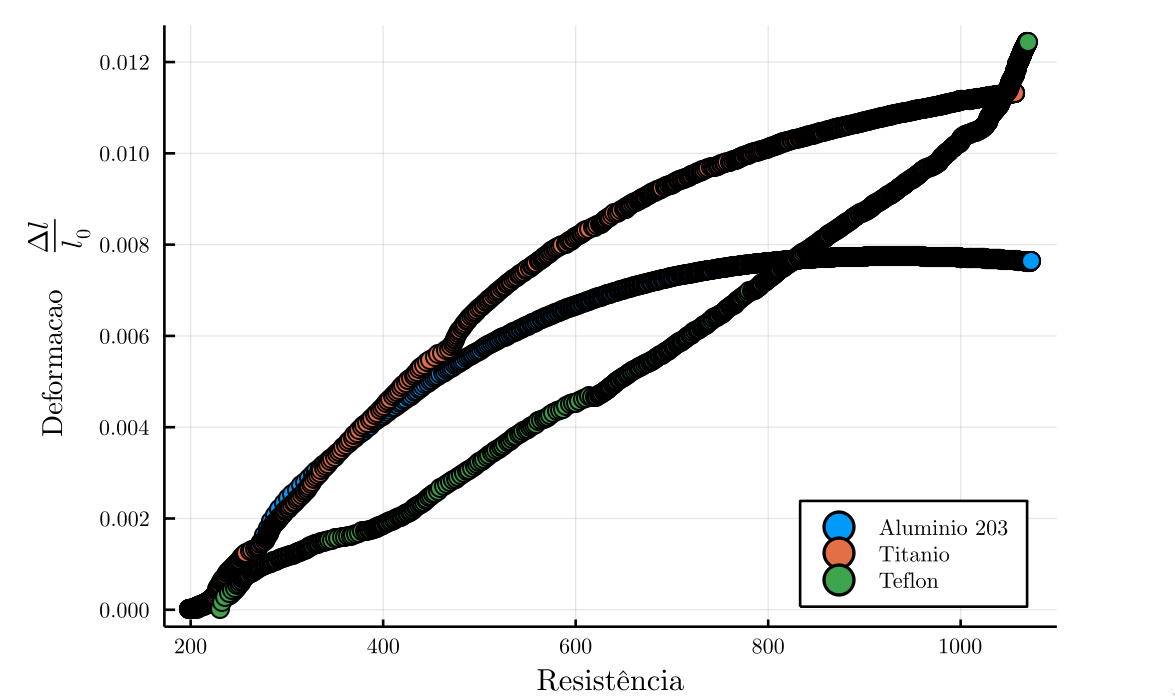
\includegraphics[width=.9\linewidth]{./img/comparacao-conjunta.png}}

\href{img/comparacao-conjunta-curva.png}{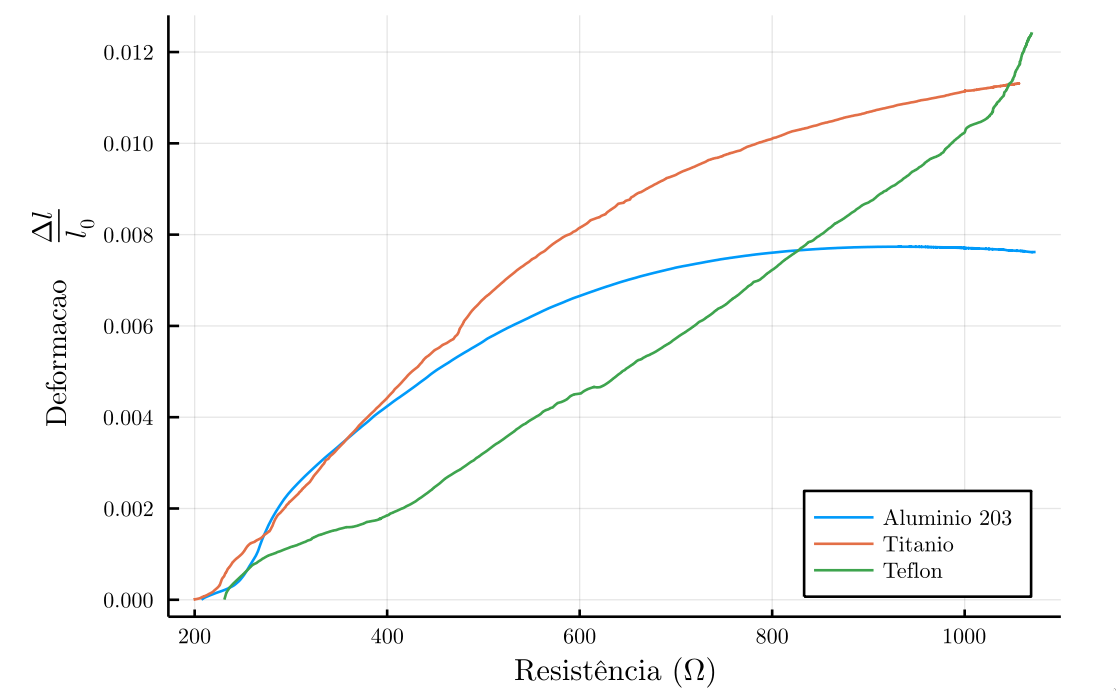
\includegraphics[width=.9\linewidth]{./img/comparacao-conjunta-curva.png}}

Escolhemos modelar as curvas com polinômios de segundo grau, \(\frac{\Delta l}{l_0}(R)\), da deformação em relação a resistência.

\subsection{Cálculo dos erros médios e o desvio padrão (resíduos)}
\label{sec:org04bf72d}

Escreveu-se uma função em Julia para o cálculo do erro médio, e o desvio padrão,

\begin{verbatim}
# poli_data is data of the polynome;
#exp_data is the experimental data.
function error_calc(poli_data,exp_data)
  sum_diff = 0
  sum_diff_2 = 0
  for i in length(exp_data)
      sum_diff += abs(poli_data[i] - exp_data[i])
      sum_diff_2 += (poli_data[i]-exp_data[i])^2
  end
  mean_sum_diff = sum_diff/2
  mean_mod_sum_diff = sqrt(sum_diff_2)/length(exp_data)
  return mean_sum_diff, mean_mod_sum_diff
end
\end{verbatim}

\subsubsection{Modelagem polinomial Alumínio 203}
\label{sec:org519b7ec}
O polinômio encontrado, para o Alumínio 203, modelando a relação \(\frac{\Delta l}{l_0}(R)\),

\begin{equation}
f(x)=-5,020239.10^{-3}(9) + 2,8813.10^{-5}(9).x - 1,6.10^{-8}(9).x^2
\end{equation}

O erro médio (módulo) e o desvio: \((\mu, \sigma)_{\textrm{erro}} = (1,12879(9).10^{-4}, 1,980.10(9)^{-7})\).

Os valores que desejamos medir são da ordem de \(10^{-3}\). Portanto, um erro de \(10^{-4}\) faz com que as medidas sejam ≅ 90\% confiáveis.

\href{img/polinomio-aluminio203.png}{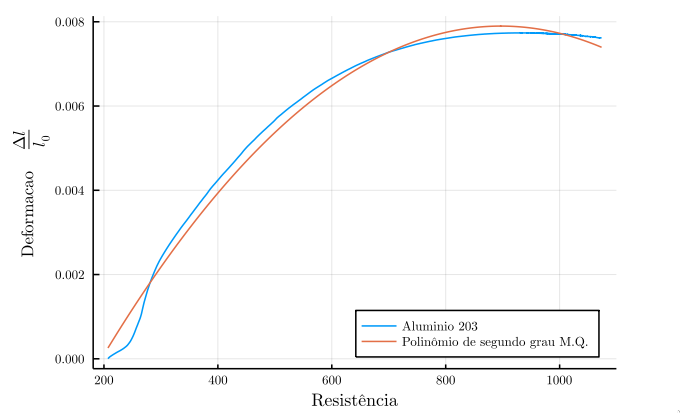
\includegraphics[width=.9\linewidth]{./img/polinomio-aluminio203.png}}

\begin{enumerate}
\item Primeira derivada do polinômio
\label{sec:org3989916}
Como o valor variante possui coeficiente da ordem \(10^{-8}\), praticamente esse valor é constante, \(2,8813.10^{-5}\). Esse seria nosso \(\alpha_{\textrm{alumínio}}\).

\begin{equation}
f'(x)=2,8813.10^{-5}(9) - 3,2.10^{-8}(9).x
\end{equation}
\end{enumerate}

\subsubsection{Modelagem polinomial Titânio}
\label{sec:org15a3677}
O polinômio encontrado, para o Titânio, modelando a relação \(\frac{\Delta l}{l_0}(R)\),

\begin{equation}
f(x)=-6,15289.10^{-4}(9) + 3.2824.10^{-5}(9).x - 1,6.10^{-8}(9).x^2
\end{equation}

O erro médio (módulo) e o desvio: \((\mu, \sigma)_{\textrm{erro}} = (4,77115(9).10^{-5}, 8,24.10(9)^{-8})\).

Os valores que desejamos medir são da ordem de \(10^{-3}\). Portanto, um erro da ordem de \(5.10^{-5}\) faz com que as medidas sejam ≅ 95\% confiáveis.

\href{img/polinomio-aluminio203.png}{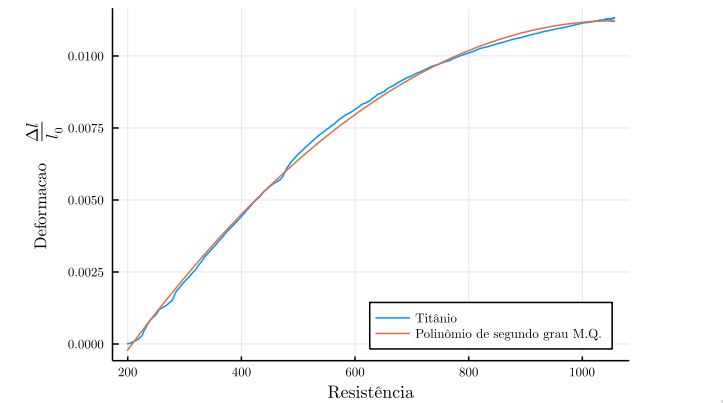
\includegraphics[width=.9\linewidth]{./img/polinomio-titanio.png}}

\begin{enumerate}
\item Primeira derivada do polinômio
\label{sec:org8cf46bd}
Como o valor variante possui coeficiente da ordem \(10^{-8}\), praticamente esse valor é constante, \(3.2824.10^{-5}(9)\). Esse seria nosso \(\alpha_{\textrm{titânio}}\).

\begin{equation}
f'(x)=3.2824.10^{-5}(9) - 3,2.10^{-8}(9).x
\end{equation}
\end{enumerate}

\subsubsection{Modelagem polinomial Teflon}
\label{sec:org0244453}
O polinômio encontrado, para o Teflon, modelando a relação \(\frac{\Delta l}{l_0}(R)\),

\begin{equation}
f(x)=-6,24966.10^{-4}(9) + 3.580.10^{-6}(9).x - 8.10^{-9}(9).x^2
\end{equation}

O erro médio (módulo) e o desvio: \((\mu, \sigma)_{\textrm{erro}} = (2,54016(9).10^{-4}, 4,38.10(9)^{-7})\).

Os valores que desejamos medir são da ordem de \(10^{-3}\). Portanto, um erro da ordem de \(2,54.10^{-4}\) faz com que as medidas sejam ≅ 90\% confiáveis.

\href{img/polinomio-aluminio203.png}{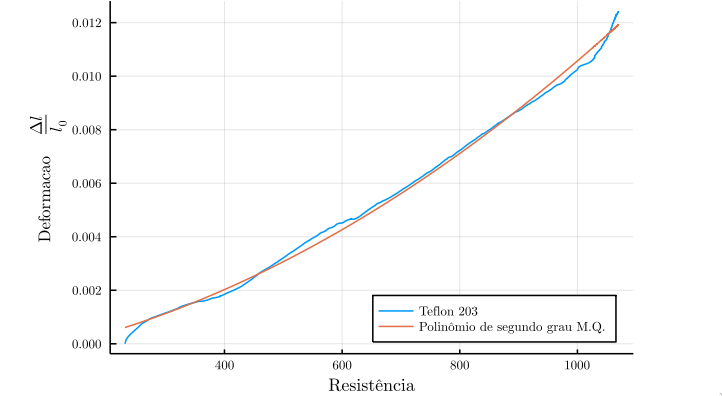
\includegraphics[width=.9\linewidth]{./img/polinomio-teflon.png}}

\begin{enumerate}
\item Derivada do Polinômio
\label{sec:org92223ec}

\begin{equation}
f(x)=-6,24966.10^{-4}(9) + 3.580.10^{-6}(9).x - 8.10^{-9}(9).x^2
\end{equation}

Como o valor variante possui coeficiente da ordem \(10^{-8}\), praticamente esse valor é constante, \(3.2824.10^{-5}(9)\). Esse seria nosso \(\alpha_{\textrm{teflon}}\).

\begin{equation}
f'(x)=3.580.10^{-6}(9) - 1,6.10^{-8}(9).x
\end{equation}

Nota-se que esse valor é uma ordem de grandeza menor do que os outros dois materiais metálicos.
\end{enumerate}

\subsubsection{Modelagem polinomial da Platina 1000}
\label{sec:orgdbcbea0}
Para Platina, utilizou-se de uma modelagem linear, pois suas medidas foram feitas entre Resistência e Temperatura. Como o aparato foi feito de forma à resistência variar exatamente conforme a temperatura varia, obteve-se uma reta.

\href{img/polinomio-aluminio203.png}{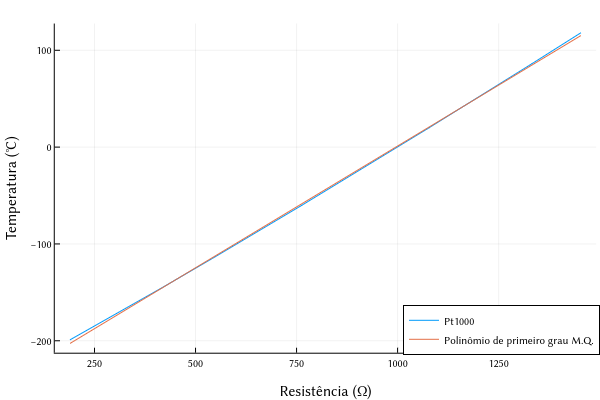
\includegraphics[width=.9\linewidth]{./img/platina.png}}

O polinômio encontrado, para a Platina, modelando a relação \(T(R)\),

\begin{equation}
f(x)=-250,407(3) + 2,52.10^{-1}(3).x
\end{equation}

O erro médio (módulo) e o desvio: \((\mu, \sigma)_{\textrm{erro}} = (1.449(3), 0.01(3))\).

As medidas possuem grandeza de \(10^3\). Assim, um erro de ordem \(10^1\) representa uma confiabilidade da ordem de ≅ 99\%.
\end{document}